
\section{H-bridge}

An H-bridge is a collecting of 4 transistors, designed to control a DC motor. In figure \ref{fig:H-bridge} the concept is illustrated. When the red switches are on, the motor runs in one direction and vica versa for the blue switches. There are two H-bridges in the system, one for the pan motor and one for the tilt motor. For further information about H-bridges, consult the \# DATASHEET H-BRO \# in the notes.




\begin{figure}[h!]
\centering
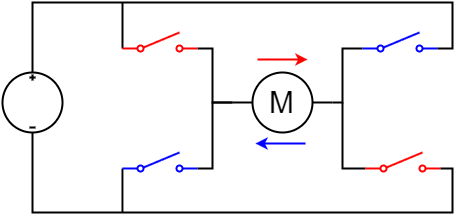
\includegraphics[scale=0.5]{Billeder/H-bridge.png}
\caption{ An example of a H-bridge }
\label{fig:H-bridge}
\end{figure}